\documentclass{article}
\usepackage{amsmath}
\usepackage{amsfonts}
\usepackage{algorithm}
\usepackage{algpseudocode}
\usepackage{graphicx}
\usepackage{hyperref}
\hypersetup{
    colorlinks=true,
    linkcolor=blue,
    filecolor=magenta,      
    urlcolor=cyan,
}
% \usepackage[linesnumbered,boxed]{algorithm2e}


% Symbols
\newcommand{\ah}{\mc{A}_{h}}
\newcommand{\ak}{\mc{A}_{k}}
\newcommand{\ahk}{\ah \cup \ak}

\newcommand{\bin}{\set{0, 1}}
\newcommand{\binbits}[1]{\bin ^{#1}}

\newcommand{\ep}[1]{epoch_{#1}}
\newcommand{\epv}{\ep{V}}
\newcommand{\epp}{(V,\accv )}

\newcommand{\gllij}{g'_{L + 1 + i - j}}
\newcommand{\gllj}{g'_{L + 1 - j}}

\newcommand{\la}{\leftarrow}
\newcommand{\lar}{\leftarrow _{R}}

\newcommand{\mb}[1]{\mathbb{#1}}
\newcommand{\mbg}[1]{\mb{G}_{#1}}
\newcommand{\mbz}[1]{\mb{Z}_{#1}^{*}}

\newcommand{\mc}[1]{\mathcal{#1}}
\newcommand{\mch}{\mc{H}}
\newcommand{\mt}[1]{\mathtt{#1}}

\newcommand{\old}[1]{{#1}^{old}}

\newcommand{\set}[1]{\{{#1}\}}
\newcommand{\range}[1]{[{#1}]}
\newcommand{\rgp}[1]{\range{1, {#1}}}
\newcommand{\rgpl}{\rgp{l}}
\newcommand{\rgptlml}{(\rgp{2L}\backslash \set{L+1})}

\newcommand{\st}[1]{state_{#1}}
\newcommand{\stv}{\st{V}}
\newcommand{\td}[1]{\tilde{#1}}

\newcommand{\vi}{V\cup \set{i}}

\newcommand{\true}{\texttt{True}}
\newcommand{\false}{\texttt{False}}

\newcommand{\ski}{sk_{I}}
\newcommand{\pki}{pk_{I}}

\newcommand{\accv}{acc_{V}}
\newcommand{\accvi}{acc_{\vi}}

\newcommand{\cp}{C_{P}}
\newcommand{\cpp}{(\group{m_i}{i}{(\ahk )}, A, e, v)}
\newcommand{\cnr}{C_{NR}}
\newcommand{\cnrp}{(I_{A}, \sigma , c, s, \witi , g_i, g'_i, i)}
\newcommand{\cpnr}{\cp , \cnr }

\newcommand{\pk}{P_{k}}
\newcommand{\pkp}{(n, S, Z, \group{R_i}{i}{\rgpl })}
\newcommand{\pr}{P_{r}}
\newcommand{\prp}{(h, h_0, h_1, h_2, \td{h}, \hat{h}, u, pk, y, z)}
\newcommand{\pl}{\mc{P}_{1}}
\newcommand{\plp}{(c, \hat{x}_{z}, \group{ \hat{x}_{r_{i}}}{i}{\rgpl })}
\newcommand{\pkip}{(\pk , \pl , \pr )}

\newcommand{\rc}{R_{c}}
\newcommand{\rcp}{(\group{m_i}{i}{\ak }, A, e, v'', s_{e}, c')}
\newcommand{\rr}{R_{r}}
\newcommand{\rrp}{(I_{A}, \sigma , c, s'', \witi , g_{i}, g'_{i}, i)}

\newcommand{\reqp}{(U, c, \hat{v}', \group{\hat{m}_{i}}{i}{\ah},n_{1}, U_{r})}
\newcommand{\resp}{(\accv ,\mc{H}, \rc , \rr )}

\newcommand{\stp}{(V, \stpp )}
\newcommand{\stpp}{\group{g_{i}, g'_{i}}{i}{\rgptlml}}

\newcommand{\setup}{\mt{setup}}
\newcommand{\setupi}{\setup(l, L)}
\newcommand{\setupp}{(\keypair{I}, \stv , \epv )}

\newcommand{\cdt}{\mt{credential}}
\newcommand{\crreq}{\cdt _{req}}
\newcommand{\crreqp}{\crreq (\mc{S}, \ah, \group{m_i}{i}{\ah}, n_0, \mc{H}, \pki )}
\newcommand{\crres}{\cdt _{res}}
\newcommand{\crresp}{\crres (i, \old{\stv }, \mc{H}, \group{m_i}{i}{\ak }, \ski , req)}
\newcommand{\crrespp}{(res , \stv ,\epv )}
\newcommand{\crfinishp}{\cdt _{finish}(\pki , \vs , req, res)}

\newcommand{\vs}{(v', s')}

\newcommand{\proofp}{\mt{proof}(\cpnr ,\pki )}

\newcommand{\vrf}{\mt{verify}}
\newcommand{\verifyph}{\vrf _{req}(\pki , req)}
\newcommand{\verifyrnr}{\vrf _{\rr }(\accv, \mc{H}, \vs , \pki , \rr )}
\newcommand{\verifycon}{\vrf _{credential}(proof, \epv )}

\newcommand{\witi}{wit_{i}}
\newcommand{\witip}{(\sigma _{i}, u_{i}, g_{i}, w, V)}

\newcommand{\commitp}{(C, D, A, \mc{G}, \mc{W}, \mc{S}, \mc{U})}
\newcommand{\openerp}{(c, \rho , \group{m_{j}}{j}{\ak}, r, s, open, open', mult, mult', tmp, tmp', r', r'', r''')}


% Equations
\newcommand{\equivmod}[3]{#1\la #2\pmod{#3}}
\newcommand{\group}[3]{\set{#1}_{\forall #2\in #3}}
\newcommand{\keypair}[1]{sk_{#1}, pk_{#1}}
\newcommand{\keypairv}[3]{sk_{#1}\la {#2}\mbox{, }pk_{#1}\la {#3}}
\newcommand{\pairing}[2]{e(#1\mbox{, }#2)}
\newcommand{\pairingexp}[3]{\pairing{#1}{#2}^{#3}}
\newcommand{\prodi}[3]{\prod _{\forall #1\in #2}#3}
\newcommand{\randexp}[4]{#1\lar \mbz{#2}\mbox{, }#3\la #4^{#1}}
\newcommand{\randexpm}[5]{\randexp{#1}{#2}{#3}{#4}\pmod{#5}}
\newcommand{\zkp}[2]{\hat{#1}_{#2}\la \td{#1}_{#2} + c\cdot #1_{#2}}
\newcommand{\zkv}[6]{\td{#1}_{#2}\la #1_{#2}^{-#3}#4^{\hat{#5}{#6}}}



\begin{document}
\title{Cryptography of Hyperledger Indy}
\author{Kyle Huang}
\maketitle

\section{Syntax of Hyperledger Indy}
The first four steps are similar to the register operation, and the last four steps look like login.\footnote{All content refers to \href{https://hyperledger-indy.readthedocs.io/projects/hipe/en/latest/text/0109-anoncreds-protocol/README.html}{Hyperledger Indy HIPE}.}
\begin{enumerate}
\item Issuer determines a credential schema $\mc{S}$: the type of cryptographic signatures used to sign the credentials, the number $l$ of attributes in a credential, the indices $\ah \subset \rgpl = \{1, 2, ..., l\}$ of hidden attributes, the public key $\pk $, the non-revocation credential attribute number $l_{r}$ and non-revocation public key $\pr $. Then he publishes it on the ledger and announces the attribute semantics.
\item Holder retrieves the credential schema from the ledger and sets the hidden attributes.
\item Holder requests a credential from issuer. He sends hidden attributes in a blinded form to issuer and agrees on the values of known attributes $\ak \la \rgpl \backslash \ah $.
\item Issuer returns a credential pair $(C_{p}, C_{NR})$ to holder. The first credential contains the requested $l$ attributes. The second credential asserts the non-revocation status of the first one. Issuer publishes the non-revoked status of the credential on the ledger.
\item Holder approaches verifier. Verifier sends the Proof Request $\mc{E}$ to holder. The Proof Request contains the credential schema $\mc{S}_{E}$ and disclosure predicates $\mc{D}$. The predicates for attribute $m$ and value $V$ can be of form $m=V$, $m<V$, or $m>V$. Some attributes may be asserted to be the same: $m_{i}=m_{j}$.
\item Holder checks that the credential pair he holds satisfies the schema $\mc{S}_{E}$. He retrieves the non-revocation witness from the ledger.
\item Holder creates a proof $\mc{P}$ that he has a non-revoked credential satisfying the proof request $\mc{E}$ and sends it to verifier.
\item Verifier verifies the proof.
\end{enumerate}

\begin{figure}
	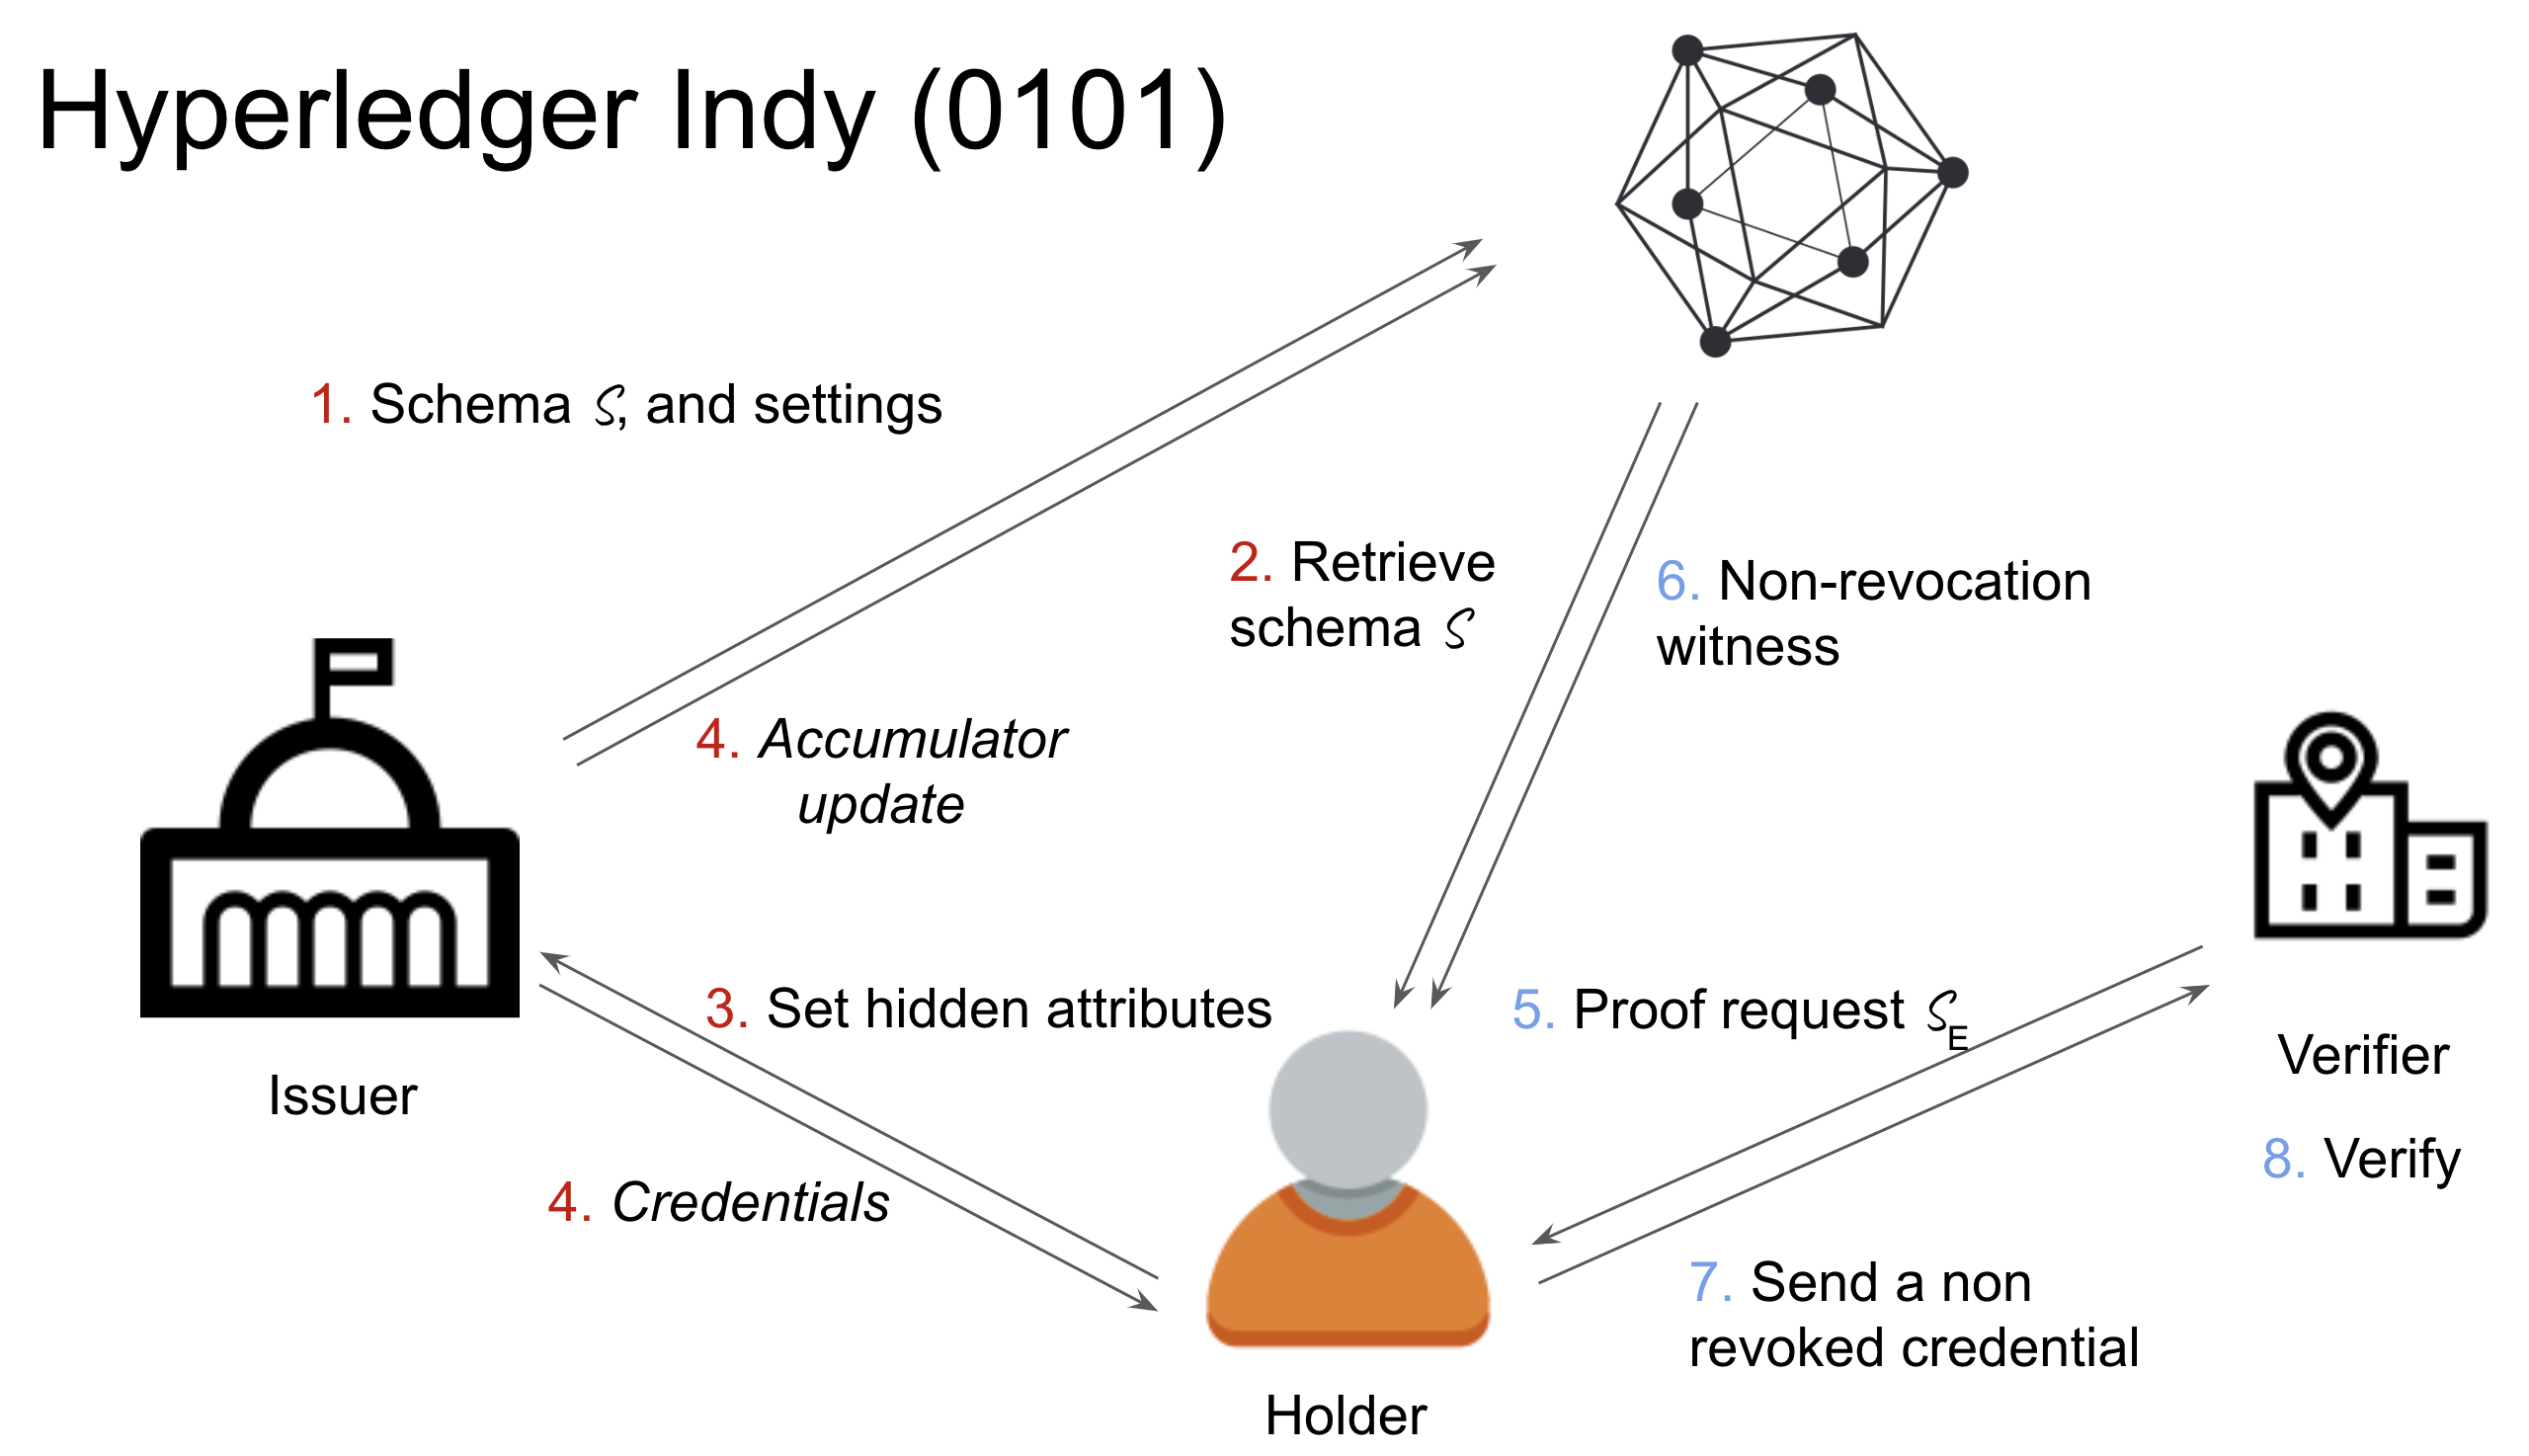
\includegraphics[width=\textwidth]{syntax.png}
	\caption{Syntax of Hyperledger Indy}
	\label{fig:indy}
\end{figure}

\begin{table}[h!]
\centering
\begin{tabular}{|c|l|} 
 \hline
 Symbol & Definition \\ \hline
 $\mc{S}$ & Schema, the empty data form with only fields. \\
 $(l, l_{r})$ & \textbf{Attributes} number and \textbf{non-revocation} credential attribute number. \\
 $L$ & The volume of a non-revocation list. \\
 $l_{a}$ & Message length for all attributes. In Sovrin, $l_{a}=256$. \\
 $(\ak, \ah)$ & The indices of \textbf{known attributes} and \textbf{hidden attributes} respectively.  \\
 & By default, $\{1, 3\}\subset \ah$ and $\{2\}\subset \ak $. \\
 $(\pk , \pr )$ & Public keys of \textbf{primary credentials} and \textbf{non-revocation credentials} resp.\\
 $\pl $ & Correctness proof of $\pk $. \\
 $(i, \mch )$ & The \textbf{index} and \textbf{identifier} of a holder in the issuer's view. \\
 $(V, \accv)$ & The \textbf{indices} and \textbf{accumulator} of the current non-revocation list.\\ 
 $(C_{P}, C_{NR})$ & The \textbf{primary credential} and the \textbf{non-revocation credential}.\\ \hline
\end{tabular}
\caption{Symbol table}
\label{table:symbol}
\end{table}
\clearpage

\section{Practical construction}
\subsection{Overview}
\begin{enumerate}
	\item $\setupp\la \setupi$
	\item $\mt{obtainCert}(\mc{U}(pk_I, \ah, \group{m_{j}}{j}{\ah }), \mc{I}(\ski, \ak, \group{m_{j}}{j}{\ak }, \old{\stv }, \old{\epv },i))$
	\begin{enumerate}
		\item Update $\ep{\vi } $ on the ledger.
		\item Holder $\mc{U}$ acqires credentials $(C_{P}, C_{NR}, \witi )$ where $C_{P}\la \mt{sign}(\ski, \group{m_{j}}{j}{\ahk })$ and $C_{NR}\la \mt{sign}(\ski, (\vi ))$.
	\end{enumerate}
	\item $\epv \la \mt{updateEpoch}()$ \# By verifier. In our case, $\epv $ is on the ledger so everyone can check.
	\item $\witi \la \mt{updateWitness}(\mc{U}(\old{\witi }), \mc{I}(\stv ))$
	\item $\true /\false \la \mt{verify}(\mc{U}(C_{P}, C_{NR}, \witi ), \mc{V}(\epv))$
\end{enumerate}

\begin{algorithm}
\caption{$\setupi$}
\label{alg:setup}
\begin{algorithmic}
	\State \Comment For primary credential
	\State $p',q'\lar \binbits{1536}$
	\Comment{$p'$ and $q'$ are prime; $|p'|=|q'|=1536$}
	\State $p\la 2p'+1$; $q\la 2q'+1$; $n\la pq$
	\Comment{$p$ and $q$ are prime}
	\State $t\lar \mbz{n}$; $\equivmod{S}{t^2}{n}$
	\State $\randexpm{x_{z}}{p'q'}{Z}{S}{n}$
	\State $\group{\randexpm{x_{r_i}}{p'q'}{R_{i}}{S}{n}}{i}{\rgpl }$
	\State $\pk \la \pkp $
	\State \Comment The proof of correctness for $\pk $
	\State $\randexpm{\td{x}_{z}}{p'q'}{\td{Z}}{S}{n}$
	\State $\group{\randexpm{\td{x}_{r_i}}{p'q'}{\td{R}_{i}}{S}{n}}{i}{\rgpl }$
	\State $c\la H_{1}(Z||\td{Z}||\group{R_i,\td{R}_i}{i}{\rgpl })$
	\Comment $H_1$ is by default SHA2-256
	\State $\zkp{x}{z}$; $\group{\zkp{x}{r_{i}}}{i}{\rgpl }$
	\State $\pl \la \plp$
	\State \Comment For non-revocation credential
	\State $\mbg{1}\times \mbg{2} \rightarrow \mbg{T}$
	\Comment pick a type-III pairing where $|\mbg{1}|=|\mbg{2}|=|\mbg{T}|=q$
	\State $g\lar \mbg{1}$; $g'\lar \mbg{2}$
	\State $h, h_0, h_1, h_2, \td{h}\lar \mbg{1}$; $u, \hat{h}\lar \mbg{2}$
	\State $sk, x, r \lar \mbz{q} $; $pk \la g^{sk}$; $y \la \hat{h}^{x}$
	\State \Comment accumulator settings
	\State $z\la \pairingexp{g}{g'}{r^{L + 1}}$; $V\la \emptyset$; $\accv \la 1$
	\State $\group{g_i\la g^{r^{i}}, g'_i\la g'^{r^{i}}}{i}{\rgptlml}$
	\State $\stv \la \stp $; $\epv \la \epp $
	\State $\pr \la \prp $
	\State $\keypairv{I}{(p, q, sk, x, r)}{\pkip }$
	\State \Return $\setupp $
\end{algorithmic}
\end{algorithm}

\begin{algorithm}
\caption{$\mt{verify}_{\pk }(l, \pk , \pl )$}
\label{alg:verifypk}
\begin{algorithmic}
	\State $\pkp \la \pk $; $\plp \la \pl $
	\State $\zkv{Z}{}{c}{S}{x}{_{z}}$; $\group{\zkv{R}{i}{c}{S}{x}{_{r_{i}}}}{i}{\rgpl }\pmod{n}$
	\State \Return $c==H_{1}(Z||\td{Z}||\group{R_i,\td{R}_i}{i}{\rgpl })$
\end{algorithmic}
\end{algorithm}

\subsection{Setup}
Issuer generates the key pair $(\keypair{I})$, $\stv $ and $\epv $ through $\setup$ (Algorithm \ref{alg:setup}); then, he keeps $(\ski, \stv )$ in a secret manner and publishes $(\mc{S}, \ah , l_{r}, \pki, \epv )$ to the ledger. Let $\pkip \la \pki$, everyone can verify the correctness of $\pk $ through $\mt{verify}_{\pk }(l, \pk , \pl )$ (Algorithm \ref{alg:verifypk}).
\begin{equation}
	\setupp \la \setupi
\end{equation}



\subsection{Credential Issuance}
\begin{align*}
	(\cpnr, \stv, \epv, \witi )&\la \mt{ObtainCert}(\mc{U}(pk_I, \ah, \group{m_{j}}{j}{\ah }), \\
	&\mc{I}(\ski, \ak, \group{m_{j}}{j}{\ak }, \old{\stv }, \old{\epv },i))
\end{align*}


Let $i<L$ and $\mch $ be the index and identifier of the holder in the issuer's system, respectively. The holder acquires the schema $\mc{S}$, indices $\ah$ and public keys $\pki$ from the ledger in addition to a random number $n_0$ and the identifier $\mch $ from the issuer; then he sets the hidden attribute $\group{m_i}{i}{\ah}$. The credential issuance process is interactive, which follows: 
\begin{enumerate}
	\item The holder requests a credential query $req$ by excuting Algorithm \ref{alg:req}, $\crreq$; then, he keeps $\vs  $ private and sends $req$ to the issuer.
	\begin{equation}
		(req, \vs) \la \crreqp
	\end{equation}
	\item On receiving $req$ from the holder, the issuer firstly verifies $req$ through $\verifyph $ (Algorithm \ref{alg:verifyreq}). If it passes, the issuer runs Algorithm \ref{alg:res}, $\crresp$, to generate parameters $\crrespp $. Finally, the issuer stores the holder’s information and index $i$ in issue’s local database, updates its own $\stv$; then, he updates $\epv$ on the ledger and returns $res$ to the holder.
	\begin{displaymath}
		\crrespp \la 
	\end{displaymath}
	\begin{equation}
		\crresp
	\end{equation}
	\item While receiving response $res$ from the issuer, the holder excutes Algorithm \ref{alg:ci3} $\crfinishp$ to do some verifications. If all verifications pass, the holder keeps returned credential $(\cpnr )$ and witness $\witi $.
	\begin{equation}
		 (\cpnr )\la \crfinishp
	\end{equation}
\end{enumerate}

\begin{algorithm}
\caption{$\crreqp$}
\label{alg:req}
\begin{algorithmic}
	\State \Comment primary credential
	\State $\group{\td{m}_i\lar \binbits{593}}{i}{\ah}$; $\pkip \la \pki$
	\State $v'\lar \binbits{3152}$; $\td{v}'\lar \binbits{3488}$
	\State $\pkp \la \pk $
	\State $U\la S^{v'}\prodi{i}{\ah}{R_{i}^{m_{i}}}$; $\td{U}\la S^{\td{v}'}\prodi{i}{\ah}{R_{i}^{\td{m}_{i}}}$
	\State $c = H(U||\td{U}||n_{0})$; $n_1\lar \binbits{80}$
	\State $\zkp{v}{}$; $\group{\zkp{m}{i}}{i}{\ah}$
	\State \Comment non-revocation credential
	\State $\prp \la \pr $
	\State $\randexp{s'}{q}{U_{r}}{h_{2}}$
	\State $req \la \reqp  $
	\State \Return $(req, \vs )$
\end{algorithmic}
\end{algorithm}

\begin{algorithm}
\caption{$\verifyph$}
\label{alg:verifyreq}
\begin{algorithmic}
	\State $\pkip \la \pki $
	\State $\pkp \la \pk $; $\reqp  \la req$
	\State $\zkv{U}{}{c}{S}{v}{'}\prodi{i}{\ah}{S^{\hat{m}_{i}}R_{i}^{-c}}\pmod{n}$
	\State \Return $c == H(U||\td{U}||n_{0})$
\end{algorithmic}
\end{algorithm}

\begin{algorithm}
\caption{$\crresp$}
\label{alg:res}
\begin{algorithmic}
	\State \Comment primary credential
	\State $\pkip \la \pki $; $m_{2}\la H(i||\mch )$
	\Comment $\mch $ is the identifier of holder, like ID
	\State $\pkp \la \pk $; $\reqp  \la req$
	\State $\td{U}\la (U^{-c}S^{\hat{v}'})\prodi{i}{\ah}{R_{i}^{\hat{m}_{i}}}$, $(p, q, sk, x, r)\la \ski $
	\If{$c\neq H(U||\td{U}||n_{0})$}
		\State \Comment And some confusing length verifications for $\hat{v}',\group{\hat{m}_{i}, \hat{r}_{i}}{i}{\ah}$ 
		\State \textbf{exit}
	\EndIf
	\State $v''\la \binbits{2724}$; $e\la 2^{596} + \binbits{119}$
	\Comment $|v''|= 2724$ and $e$ is prime
	\State $Q\la Z(US^{v''}\prodi{i}{\ak}{R_{i}^{m_{i}}})^{-1}\pmod{n}$
	\State $A\la Q^{e^{-1}\pmod{p'q'}}$; $r\lar \mbz{p'q'}$; $\hat{A}\la Q^{r}\pmod{n}$
	\State $c'\la H(Q||A||\hat{A}||n_{1})$; $s_{e}\la r -c'e^{-1}\pmod{p'q'}$
	\State $\rc \la \rcp$
	\State \Comment non-revocation credential
	\State $s'', c\lar \mbz{q}$; $(\old{V}, \stpp )\la \old{\stv }$
	\State $\prp \la \pr $
	\Comment $i$: the index of user on accumerlator
	\State $\sigma \la (h_{0}h_{1}^{m_{2}}U_{r}g_{i}h_{2}^{s''})^{(x+c)^{-1}}$; $\sigma _{i} \la g'^{(sk + r^{i})^{-1}}$; $u_{i}\la u^{r^{i}}$
	\State $w\la \prodi{j}{V, j\neq i}{\gllij }$; $V\la \old{V}\cup \set{i}$, $\accv \la \prodi{j}{V} \gllj$
	\State $\witi \la \witip $; $\rr \la \rrp $
	\State \Comment $I_{A}$: identifier of accumerlator
	\State $res \la \resp $
	\State $\stv \la \stp $; $\epv \la \epp $
	\State \Return $\crrespp $
\end{algorithmic}
\end{algorithm}

\begin{algorithm}
\caption{$\crfinishp $}
\label{alg:ci3}
\begin{algorithmic}
	\State $\pkip \la \pki $; $\pkp \la \pk $; 
	\State $\prp \la \pr $
	\State $\reqp \la req$; $\resp \la res$
	\State $\rcp \la \rc $; $\rrp \la \rr $
	\State $\witip \la \witi$; $m_2\la H(i||\mch )$
	\State $v\la v' + v''$; $s\la s' + s''$
	\State $Q\la Z(S^{v}\prodi{i}{(\ak \cup \ah)}{R_{i}^{m_{i}}})^{-1}\pmod{n}$
	\State $\hat{A}\la A^{c'+s_{e}\cdot e}$
	\If{$\pairing{g_{i}}{\accv }(\pairing{g}{w})^{-1}\neq z$}
		\State \Return \textbf{null}
	\ElsIf{$\pairing{pk\cdot g_{i}}{\sigma _{i}}\neq \pairing{g}{g'}$}
		\State \Return \textbf{null}
	\ElsIf{$\pairing{\sigma }{y\cdot \hat{h}^{c}}\neq \pairing{h_{0}h_{1}^{m_{2}}h_{2}^{s}\cdot g_{i}}{\hat{h}}$}
		\State \Return \textbf{null}
	\ElsIf{$e$ is not prime OR $e\not \in [2^{596}, 2^{596} + 2^{119}]$}
		\State \Return \textbf{null}
	\ElsIf{$Q\neq A^{e}$}
		\State \Return \textbf{null}
	\ElsIf{$c'\neq H(Q||A||\hat{A}||n_{1})$}
		\State \Return \textbf{null}
	\Else \State $\cp \la \cpp$; $\cnr \la \cnrp$
	\State \Return $(\cpnr )$
	\EndIf
\end{algorithmic}
\end{algorithm}

\subsection{Credential Revocation}
The revocation process is quite straightforward. The issuer fetches the current $\old{\epv }$ from the ledger. Then, he revokes user with index $i$ via Algorithm \ref{alg:revoke} and updates $\epv $ and $\stv$ on the ledger and in its private database, respectively, after running $(\stv ,\epv )\la \mt{revoke}(\old{\epv}, i)$. 

\begin{algorithm}
\caption{$\mt{revoke}(\old{\stv}, \old{\epv }, i)$}
\label{alg:revoke}
\begin{algorithmic}
	\State $(\old{V}, \stpp )\la \old{\stv }$; $(\old{V}, \old{\accv })\la \old{\epv }$
	\State $V \la \old{V} \backslash \{i\}$; $\accv \la \old{\accv }\cdot (\gllj)^{-1}$
	\State $\stv \la (V, \stpp)$;  $\epv \la (V, \accv )$
	\State \Return $(\stv ,\epv )$
\end{algorithmic}
\end{algorithm}

\subsection{Epoch update}
The epoch update is omitted since the epoch is stored on the ledger in Hyperledger Indy so that each node synchronizes the last version of epoch.

\subsection{Witness update}
While a verifier touches a holder to issue a zero-knowledge proof, the first step of the holder is to update his witness by requesting $\old{\witi }$ to the issuer; and the issuer computes and returns through $\mt{WitnessUpdate}$ (Algorithm \ref{alg:witupdate}).

\begin{algorithm}
\caption{$\mt{updateWitness}(\old{\witi }, \stv)$}
\label{alg:witupdate}
\begin{algorithmic}
	\State $(\sigma _{i}, u_{i}, g_{i}, \old{w}, \old{V})\la \old{\witi }$; $\stp \la \stv$
	\State $w \la \old{w} \prodi{j}{V \backslash \old{V}}\gllij / \prodi{j}{\old{V} \backslash V}\gllij $
	\State $\witi \la (\sigma _{i}, u_{i}, g_{i}, w, V)$
	\State \Return $\witi $
\end{algorithmic}
\end{algorithm}

\subsection{Credential verification}
After updating the witness, the holder generates a $proof\la \proofp $ (algorithm \ref{alg:proof}). Let $(commit, opener)\la proof$ be the generated proof, the holder sends $commit$ to the verifier first, after confirmation from the verifier, the holder sends $opener$ to the verifier to open the aforementioned $commit$; and the verifier is convinced if algorithm \ref{alg:verifycre} returns $\true \la \verifycon $.

\begin{algorithm}
\caption{$\proofp $}
\label{alg:proof}
\begin{algorithmic}
	\State $\cpp \la \cp$; $\cnrp \la \cnr$
	\State $\witip \la \witi $; $\pkip \la \pki $
	\State $\prp \la \pr $; $\rho , r, r', r'', r''', \lar \mbz{q}$
	\State $mult\la c\rho $; $tmp\la c \cdot open$; $mult'\la r''\cdot r$; $tmp'\la r'' \cdot open$
	\State $C\la h^{\rho }\td{h}^{open}$; $D\la g^{r}\td{h}^{open'}$; $A\la \sigma \td{h}^{\rho }$; $\mc{G}\la g_{i}\td{h}^{r}$
	\State $\mc{W}\la wg'^{r'}$; $\mc{S}\la \sigma _{i}g'^{r''}$; $\mc{U}\la u_{i}g'^{r'''}$
	\State $commit\la \commitp $ 
	\State $opener\la \openerp $
	\State $proof\la (commit, opener)$
	\State \Return $proof$
\end{algorithmic}
\end{algorithm}

\begin{algorithm}
\caption{$\verifycon $}
\label{alg:verifycre}
\begin{algorithmic}
	\State $(commit, opener) \la proof$; $\commitp \la commit$
	\State $\openerp \la opener $
	\State $\epp \la \epv $
	\State $X_{1}\la \pairing{h_{0}\cdot \prodi{j}{\ak}{h_{j}^{m_{j}}}\cdot \mc{G}}{\hat{h}}$
	\State $X_{2}\la \pairing{A}{y\hat{h}^{c}}\pairing{\td{h}}{\hat{h}^{r-mult}y^{-\rho }}$
	\If{$C\neq h^{\rho }\td{h}^{open}$}
		\State \Return $\false$
	\ElsIf{$1\neq C^{c}h^{-mult}\td{h}^{-tmp}$}
		\State \Return $\false$
	\ElsIf{$X_{1}\neq X_{2}\cdot \prodi{j}{\ah}{\pairingexp{h_{j}}{\hat{h}}{-m_{j}}}\cdot \pairingexp{h_{l+1}}{\hat{h}}{-s}$}
		\State \Return $\false$
	\ElsIf{$\pairing{\mc{G}}{\accv}\neq \pairing{g}{\mc{W}}\cdot z\cdot \pairingexp{\td{h}}{\accv }{r}\pairingexp{g^{-1}}{g'}{r'}$}
		\State \Return $\false$
	\ElsIf{$D\neq g^{r}\td{h}^{open'}$}
		\State \Return $\false$
	\ElsIf{$1\neq D^{r''}g^{-mult'}\td{h}^{-tmp'}$}
		\State \Return $\false$
	\ElsIf{$\pairing{pk\cdot \mc{G}}{\mc{S}}\neq \pairing{g}{g'}\pairingexp{pk\cdot \mc{G}}{g'}{r''}\pairingexp{\td{h}}{g'}{-mult'}\pairingexp{\td{h}}{\mc{S}}{r}$}
		\State \Return $\false$
	\ElsIf{$\pairing{\mc{G}}{u}\neq \pairing{g}{\mc{U}}\pairingexp{\td{h}}{u}{r}\pairingexp{g^{-1}}{g'}{r'''}$}
		\State \Return $\false$
	\Else
		\State \Return $\true$
	\EndIf
\end{algorithmic}
\end{algorithm}

\end{document}
